\chapter{Le \emph{behavioral biometrics} come futuro dell'autenticazione}
Nel corso della tesi è stato fatto riferimento più volte a typingDNA e alle behavioral biometrics. Ma cosa sono esattamente? Quali sono le applicazioni e le potenzialità in termini di sicurezza informatica? Questo capitolo si occuperà di rispondere a queste domande.\\

\section{Cosa si intende con behavioral biometrics}
Le behavioral biometrics, in italiano parametri biometrici comportamentali, sono dati relativi all'uso che ogni persona fa dei suoi dispositivi, concentrandosi più su \emph{come} vengono svolte determinate azioni, che su \emph{quali} esse siano.\\
Per esempio, quasi ogni possessore di un dispositivo elettronico ha accesso ad un qualche servizio di posta elettronica e probabilmente controllerà ogni giorno le nuove email ricevute e a vote ne scriverà di sue. Ma è molto probabile che non tutti gli utenti di tale servizio aprano le email con la stessa velocità, scorrano con la rondella del mouse o col dito allo stesso modo, abbiano la stessa rapidità e accuratezza nel digitare sulla tastiera.\\
Con l'utilizzo sempre maggiore del \emph{machine learning} e dell'intelligenza artificiale è possibile immagazzinare ed elaborare le informazioni elencate sopra (e molte altre) per costruire un profilo univoco della persona che utilizza tali servizi.\\
I classici metodi per tenere in sicurezza i propri account sono ormai decadenti. Le password molto raramente vengono scelte con criteri di sicurezza elevati e comunque molti utenti decidono di salvarle all'interno del browser o attraverso un servizio di memorizzazione password. Accedendo al servizio principale sarebbe quindi possibile accedere a tutte le password dell'utente con conseguenze evidentemente gravi.\\
L'autenticazione a due fattori, che viene sempre più utilizzata, fornisce un alto livello di sicurezza, ma comunque richiede dei passaggi attivi da parte dell'utente, per essere applicata e non sarebbe pratico richiederla per ogni accesso ad un servizio.\\
Anche i parametri biometrici veri e propri (scansione dell'impronta digitale, del volto, dell'iride) sono metodi di autenticazione sicurissimi, ma richiedono componenti hardware specifiche e non sono utilizzabili in ogni situazione con comodità.\\
Se, invece, i dispositivi fossero in grado di riconoscere il proprio possessore confrontando il suo comportamento attuale con quello avuto in passato (o ancora meglio, riconoscere un tentativo di utilizzo da parte di un individuo esterno), allora potrebbe essere sempre possibile verificare l'identità dell'utente senza che lui debba compiere alcun gesto se non quelli che aveva già previsto di dover compiere. Questo sistema permetterebbe ai dispositivi e ai servizi di essere molto più \emph{user friendly}.\\
C'è da dire che costruire un profilo comportamentale per ogni individuo può spaventare molte persone, ma è opportuno tener presente che attualmente già vengono registrate molte informazioni personali su di noi. I movimenti tracciati via GPS, i passi che effettuiamo ogni giorno e potenzialmente anche il nostro modo di camminare, i battiti cardiaci e tanto altro. Sicuramente però utilizzare i dati personali comportamentali nei modi suddetti può contribuire alla sicurezza di questi stessi dati!


\section{Il servizio TypingDNA}
All'interno di \emph{Game on} ho deciso di utilizzare il servizio TypingDNA\cite{tdna} perché fornisce una dimostrazione molto semplice, ma efficace, delle potenzialità nell'utilizzo delle behavioral biometrics.\\
Con TypingDNA è possibile riconoscere un utente attraverso il suo modo di digitare su una tastiera (sia su desktop che su smartphone).\\
Il suo utilizzo è molto semplice: 
\begin{itemize}
    \item Lato client viene registrato lo stile di digitazione dell'utente grazie alla libreria javascript \emph{typingdna.js}. I parametri vengono salvati sotto forma di \emph{pattern}.
    \item Lato server il pattern ottenuto viene preso e rilanciato attraverso una chiamata REST alla REST API sui server di TypingDNA.
    \item TypingDNA risponde con un json che comunicherà la validità o meno del pattern fornito
\end{itemize}
\begin{figure}[hbt!]
    \centering
    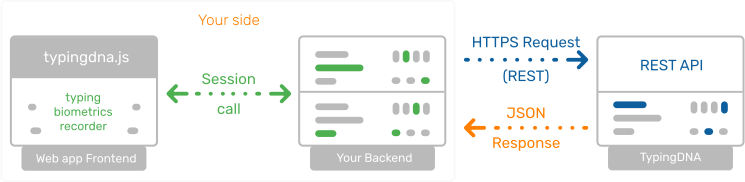
\includegraphics[width=\textwidth]{typingDNA_workflow}
    \caption{Workflow di TypingDNA}
\end{figure}
\FloatBarrier
Le API messe a disposizione permettono di verificare tre tipi di pattern: \emph{same text} autentica basandosi sulla digitazione dello stesso testo; \emph{any text} autentica basandosi sulla digitazione di testi sempre diversi; \emph{extended text} è una combinazione dei precedenti.
\subsection{Utilizzo di TypingDNA all'interno dell'applicazione}
All'interno di Game on sono stati implementati diversi controlli attraverso typingDNA: 
\begin{itemize}
    \item Un pattern \emph{same text} viene utilizzato con la mail dell'utente nei primi accessi al sito e successivamente ogni 10 login. L'utente ha 3 tentativi per entrare, dopo i quali l'account viene bloccato e una mail di recupero viene inviata all'utente.
    \item Un pattern \emph{any text} viene creato quando un utente scrive una recensione o la descrizione di un gioco e la lunghezza del testo è sufficientemente lunga. In caso di fallimento l'utente è sospetto e viene reindirizzato alla pagina di inserimento mail descritta sopra.
\end{itemize}